% !TeX root = ../thuthesis-example.tex

\chapter{THE PLATFORM USAGE IN EXTERNAL PROJECTS}

Tsinghua students, who took the Autumn 2020 HCIT course, needed to present a course project in the end of the semester. Students needed to provide research on an interaction method in a specific smart environment simulated in Virtual reality. Each team was given an Oculus Quest 2 VR headset for testing their demos. At the time of development of the coursework, students had access to the previous version of NUIX-Studio platform based on the prototype number 4. As mentioned in the previous chapter, this prototype did not have the functionality of convenient creation of devices, simultaneous work and integration of the most of IoT devices from the real world. However, the platform provided tools for interaction with virtual IoT devices. Students integrated the platform into their projects written in Unity by adding Widgets such as Sight Sensor, gesture recognition, video streaming, and virtual controls, and tested various hypotheses for interacting with devices in Virtual reality. As a result, the platform helped to achieve quite useful results in the course projects of students.

For better understanding, each project is presented in the form Subject of research - Experiment - Results. 

\section{Autumn Semester Student Course Projects}

\subsection{A comparative study of equipment positioning based on spatial location and sound feedback}

Team members:
\begin{enumerate}
    \item Liang Wenjie
    \item Wang Zixuan
    \item Sun Shikun
    \item Saito Fumiki
\end{enumerate}


\subsubsection{Subject of research}

Many people encounter the situation of not being able to find a mobile phone. Usually, people can only determine the approximate location of the mobile phone, and it is difficult to quickly specify the exact location of the device. 
In some situations, for example when preparing for an exam, traveling, etc., people need to search for multiple devices at the same time. Searching for a single device at once may not be effective.
This team introduced influencing factors such as spatial location and voice feedback to design a more convenient interaction method for device positioning in Smart home scenarios. 

\subsubsection{Experiment}
The team implemented two single device positioning methods:
\begin{enumerate}
    \item Baseline scheme: basic positioning of the device based on the stereo sound;
    \item Team solution: positioning of the device based on the spatial location and sound changes: when the angle between the user's current orientation and the user-device connection direction is smaller, the volume is louder. This can help users significantly reduce the time to find the target device. 
\end{enumerate}

9 students participated in the experiment. Each time the single device was placed in the virtual NUIX-Studio Smart home environment. The experiment participants were asked to be find the device by using each of the two positioning methods.(Figure~\ref{fig:Project1-1-figure}).

\begin{figure}
  \centering
  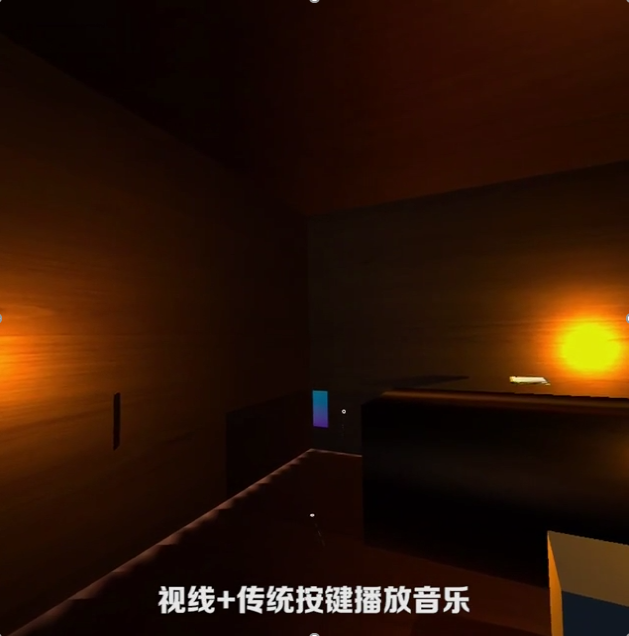
\includegraphics[width=0.9\linewidth]{figures/Project_1-1.png}
  \caption{Screenshot of the project demo.}
  \label{fig:Project1-1-figure}
\end{figure}

In the second experiment, multiple device position methods were tested:
\begin{enumerate}
    \item Baseline scheme: basic positioning of the devices based on the stereo sound;
    \item Team solution: Positioning interaction based on spatial position and voice feedback prompts. Each The object reports its spatial position by voice commands. If it is in the same room as the user, the position relative to the user will be reported. If the current object is closer to the previous object, the position relative to the previous object is reported. It can help users significantly improve the efficiency of continuously searching for different target devices in a multi-device context.
    \item Improvement: Considering people’s habit of searching for objects, large objects (such as TVs, refrigerators, etc.) are easy to find at a glance; therefore, the indexing algorithm is improved to sort the object by distance and volume.
\end{enumerate}

10 students participated in the experiment. Each time they were asked to search for the devices using the baseline and team solutions, and then give a score to each of the solutions based on the interaction efficiency, learning cost, fatigue level, and user experience. 

\subsubsection{Results}

For the first experiment, students have collected the following results:
\begin{enumerate}
    \item It can be seen that the average time used in the experimental group is generally about 15s lower than the baseline (Figure~\ref{fig:Project1-figure});
    \item On the extreme value, the experimental group has a maximum value of about 110s, which is much slower than the baseline. The Test group time was affected by the two factors of distance/angle, which made it difficult for the subject to distinguish the distance.
\end{enumerate}

\begin{figure}
  \centering
  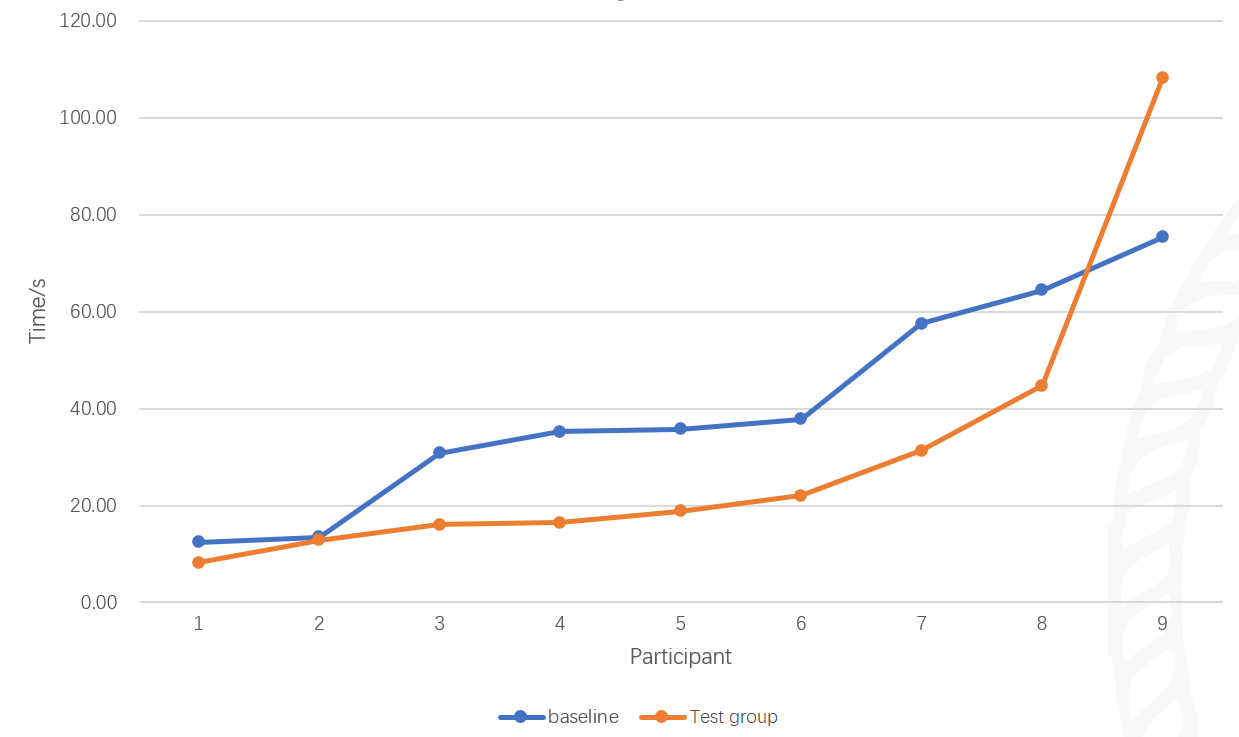
\includegraphics[width=0.9\linewidth]{figures/Project_1.png}
  \caption{Statistics and analysis of user experiment results: objective comparison experiment (single object. Single device positioning time.}
  \label{fig:Project1-figure}
\end{figure}

In the second experiment most of the users mentioned that the interaction efficiency has significantly improved by using the Team solution. However, in terms of learning costs and fatigue levels, there is little difference, because processing the sound information for finding objects is not as direct as using visual information. 

\subsection{The trigger mechanism of device switching in the Smart home scenario}

Team members:
\begin{enumerate}
    \item Huang Yanwen 
    \item Liu Wei 
    \item Liu Niqi 
    \item Zhang Xueying 
\end{enumerate}

\subsubsection{Subject of research}

People often use multiple devices with similar functionality. For example, TVs, computers, and mobile phones all have screens. The traditional methods to switch a certain display content from one device to another include using buttons, remote controls, etc. This team explored more novel triggering methods to provide users a more natural, comfortable experience.
The first method is based on using the Sight sensor Widget. When the user's line of sight intersects with a specific display for a certain period of time, the line of sight sensor will trigger.
The second method is based on using a location Widget. The sensor triggers within a certain the distance between the user and the screen.
The third method is based on the gesture recognition Widget. Users use "grab" and "throw" gestures to move content from display to another. 
The fourth method is based on button Widgets, which users can press to switch between the displays.

\subsubsection{Experiment}

The students conducted comparison and analysis of the developed trigger methods through evaluation experiments.(Figure~\ref{fig:Project2-figure}).

\begin{figure}
  \centering
  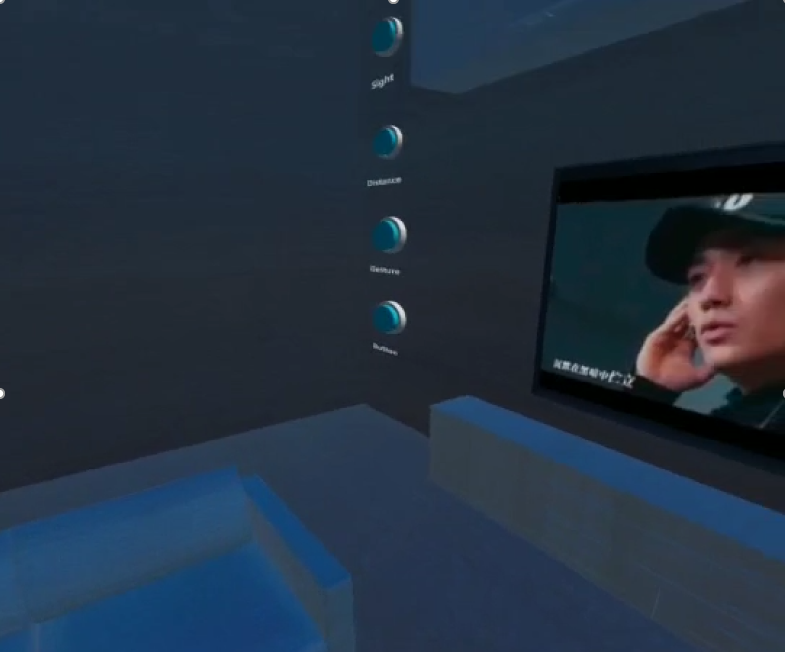
\includegraphics[width=0.9\linewidth]{figures/Project_2.png}
  \caption{Demo of the project.}
  \label{fig:Project2-figure}
\end{figure}

\subsubsection{Results}

The easiest to use method is sight-based interaction(Figure~\ref{fig:Project10-figure}), while the gesture-based provides the most naturalness, sense of control and user satisfaction.

The failure rate of gesture recognition is 5 percent. A large part of the reason is the instability of the device's hands recognition.
The user's low evaluation of button control is mainly due to the lack of actual tactile feedback in VR and unstable hand recognition, which makes the triggering of the button failed to be successfully pressed or double-clicked.
The basis for rapid device switching is the remote interconnection of multiple devices. Although the current Smart home environments have not fully achieved this goal, the team believes this is an inevitable trend in the future.\footnote{In the final prototype of NUIX-Studio, researchers can implement remote interconnection between real and virtual devices by using the Video Streaming Widget}


\begin{figure}
  \centering
  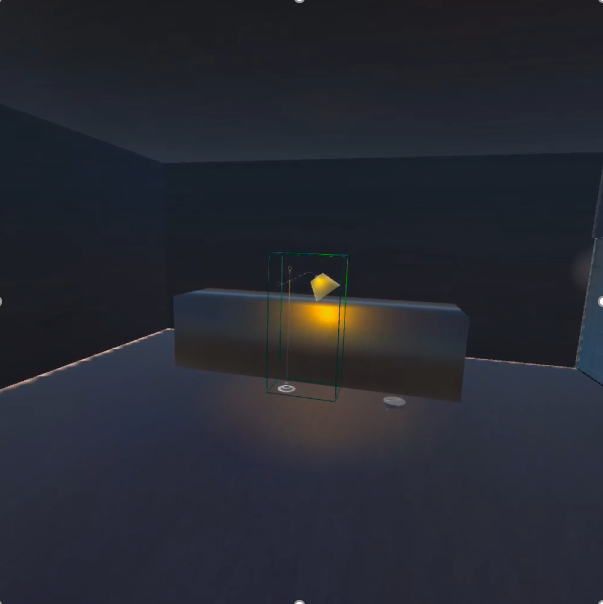
\includegraphics[width=0.9\linewidth]{figures/Project_10.png}
  \caption{Demo of another team project. By exploring the meaning of sight awakening, students Wei Tong, Chen Bohan, Lu Mengying and Zou Tianyuan developed a sight interaction method based on statistical models. }
  \label{fig:Project10-figure}
\end{figure}

\subsection{Smart gloves - New interactive devices in smart medical scenarios}

Team members:
\begin{enumerate}
    \item Deng Bowen 
    \item Niu Haoyu
    \item Wang Shijie 
    \item Zhou Huanhai 
\end{enumerate}


\subsubsection{Subject of research}

In hospitals, patients are often restricted in their activities, and cannot easily complete operations such as turning on and off lights and adjusting beds by themselves. For doctors and nurses, some actions are suitable for remote and sanitary isolation operations.

This team designed a new type of interaction method based on using smart gloves. Wearing smart gloves, user can interact with devices through gestures and hand movements. This interaction method has a wide range of application scenarios in Smart medical environment. 

\subsubsection{Experiment}

The team has added several gestures support into the gesture recognition Widget, and added those gestures to the demo to control the object Widgets inside a virtual hospital (Figure~\ref{fig:Project4-figure}).

\begin{figure}
  \centering
  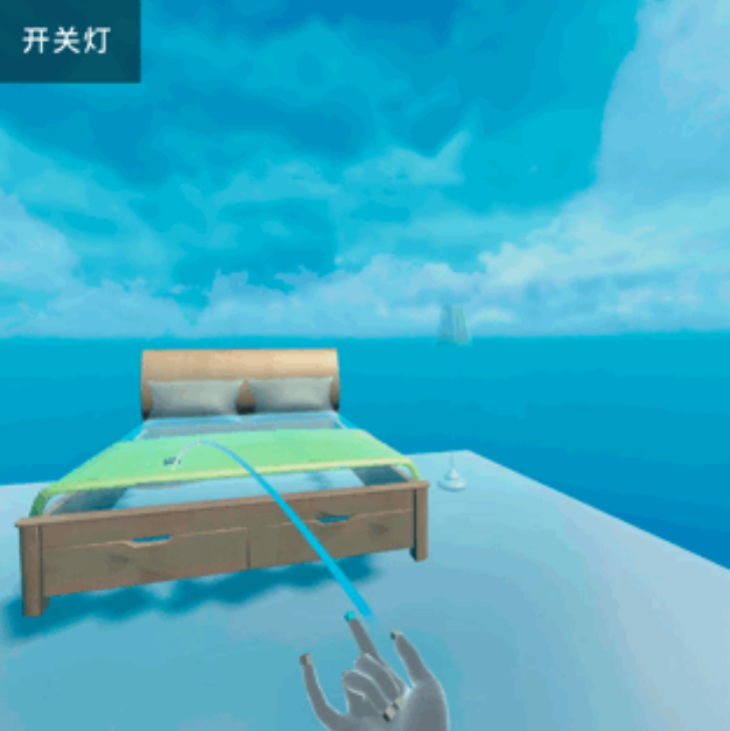
\includegraphics[width=0.9\linewidth]{figures/Project_4.png}
  \caption{One of the gestures developed. Use gesture similar to ‘Spider-Man’ (right middle finger and ring finger) to trigger the light switch.}
  \label{fig:Project4-figure}
\end{figure}

\subsubsection{Results}
Four parameters were evaluated through the user study: ease of use, interaction efficiency, fatigue and practicality. Each of the users found the demo easy to use, efficient and practical, but most of them felt moderately tired after a 5 minute experiment.

\subsection{Research on Feedforward of Home Appliance Control Based on MRTK}

Team members:
\begin{enumerate}
    \item Li Ziang
    \item Li Ao
    \item Sui Weiyi
\end{enumerate}

\subsubsection{Subject of research}

It is difficult for users to remember the mapping relationship between gestures and home appliance functions.
Solution is to add visual feed forward and trigger prompts by using a Sight Widget.

\subsubsection{Experiment}

Participants used the Smart home environment and a Gesture recognition Widget from NUIX-Studio to test the ease of learning of the demo (Figure~\ref{fig:Project7-figure}). The users needed to complete multiple tasks within 5 minutes without providing any prior knowledge in the experiment.
Next, completion rate and user ratings were collected and analyzed.

\begin{figure}
  \centering
  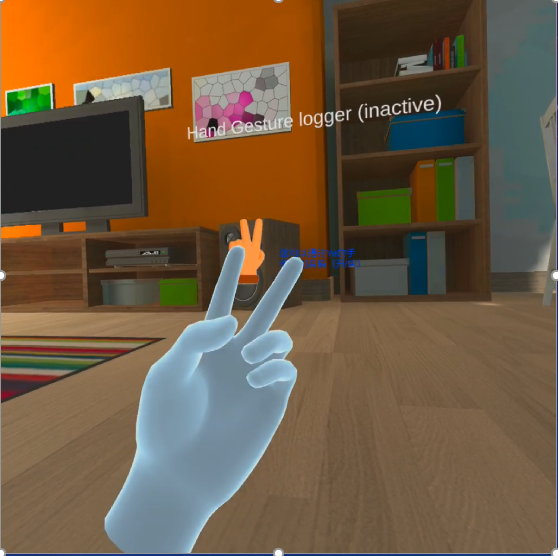
\includegraphics[width=0.9\linewidth]{figures/Project_7.png}
  \caption{Combine sight detection and gesture recognition
When the fixation time exceeds the threshold, a prompt will pop up.}
  \label{fig:Project7-figure}
\end{figure}

\subsubsection{Results}

Average score: 4.14 points (out of 5 points)
Average task completion rate: 65.29\%

\subsection{Gesture laser pointer}

Team members:
\begin{enumerate}
    \item Wang Haoyu
    \item Zhang Zeyuan 
    \item Zhang Zizhao
\end{enumerate}


\subsubsection{Subject of research}
On the podium, teachers can use computers and writing pads to mark content conveniently, but they are far away from students, what makes the interaction between them weak.
Standing next to the desks, the students and teacher get closer, but without the computer and writing board, it is difficult for the teachers to mark content effectively.
Can the function of the laser pointer be extended so that teachers can effectively mark content? 

This team has developed a gesture laser pointer based on the gesture recognition Widget, that does not need to be held in hand.
The developed tool can perform the functions of lighting, drawing rectangles, drawing circles and erasing content.

\subsubsection{Experiment}

Experimental procedure: draw rectangles in large fonts, draw circles in large fonts, draw rectangles in small fonts, draw circles in small fonts, draw lines (Figure~\ref{fig:Project9-figure}). 

\begin{figure}
  \centering
  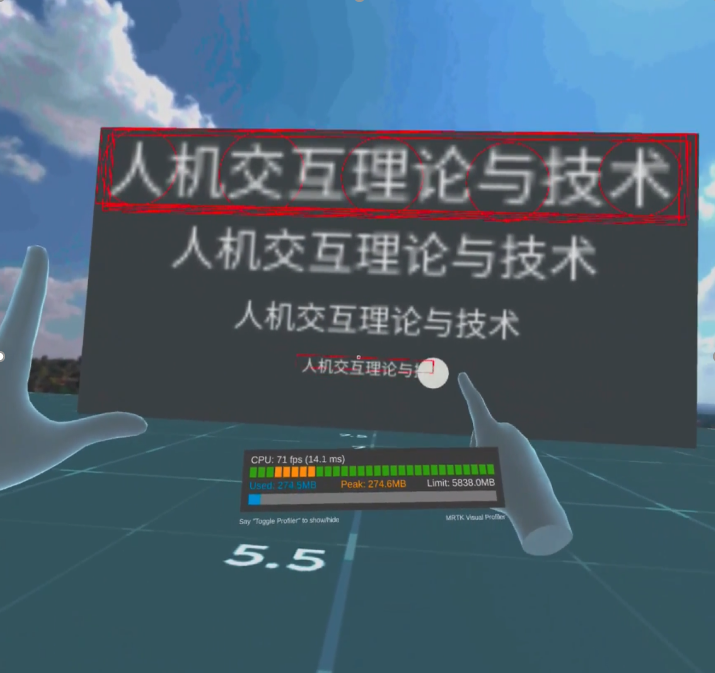
\includegraphics[width=0.9\linewidth]{figures/Project_9.png}
  \caption{Video demonstration-and user experiment process.}
  \label{fig:Project9-figure}
\end{figure}


\subsubsection{Results}

The average time to perform an experimental task varied from 3 to 5 seconds. The accuracy of drawing varied from 87.5\% to 97.5\%.

The average user satisfaction score is 8.46 points out of 10 points.

Overall the team has implemented a good instrument, which can be added to NUIX-Studio as a Widget for Smart classroom environment.

\subsection{FloorUI—home control system based on interactive ground}

Team members:
\begin{enumerate}
    \item Zhang Xiaoyu
    \item Zhu Yihao
    \item Xie Yuqing
    \item Zhang Yizhuo
\end{enumerate}


\subsubsection{Subject of research}

In this project the students explored the operation of equipment in a hands-free manner by setting a wake-up UI interface on the floor (Figure~\ref{fig:Project11-figure}). .

\begin{figure}
  \centering
  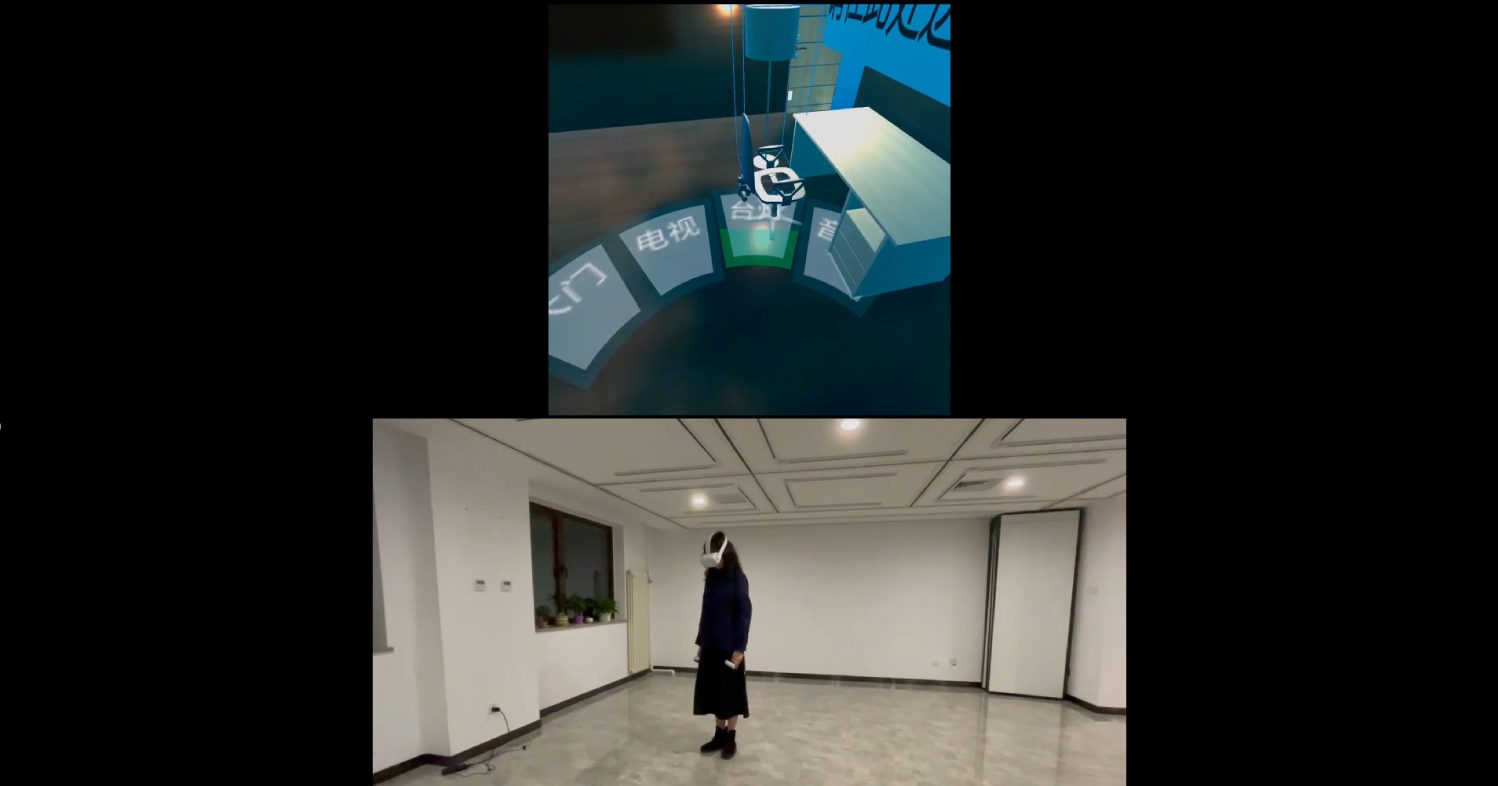
\includegraphics[width=0.9\linewidth]{figures/Project_11.png}
  \caption{Demo of the experiment.}
  \label{fig:Project11-figure}
\end{figure}

\subsubsection{Experiment}

Two different ways of interaction with the UI were tested:
\begin{enumerate}
    \item Gaze interaction. The UI element is selected by the user's gaze point. Each of the buttons can be pressed by triggering a corresponding Sight sensor Widget.
    \item Body interaction. The UI element is selected by the user's positioning of the feet (Figure~\ref{fig:Project11_1-figure}). By streaming the camera from the phone to Unity (Figure~\ref{fig:VideoStreamingWidget-figure}), the virtual location of the feet is calculated.
\end{enumerate}


\begin{figure}
  \centering
  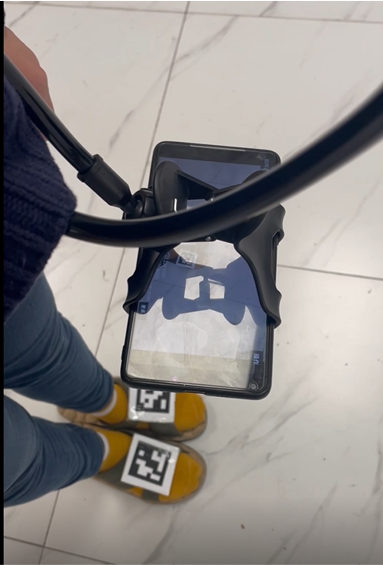
\includegraphics[width=0.6\linewidth]{figures/Project_11_1.png}
  \caption{Get the position of feet by placing a QR code on the shoes.}
  \label{fig:Project11_1-figure}
\end{figure}


\begin{figure}
  \centering
  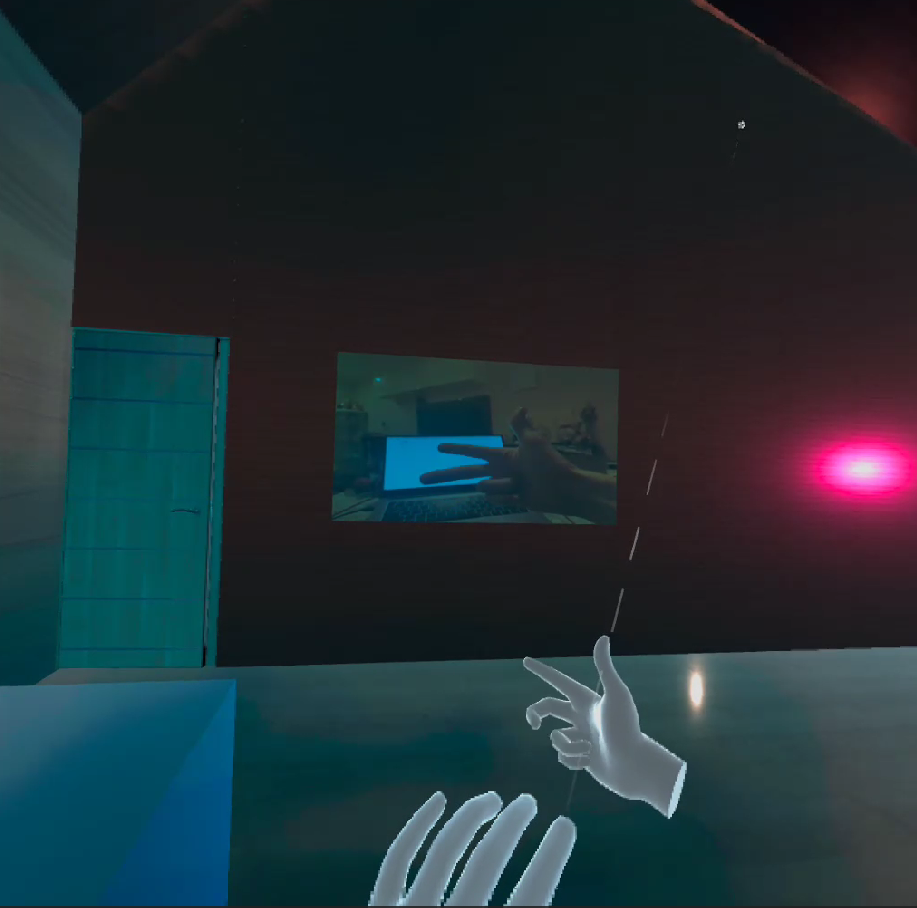
\includegraphics[width=0.9\linewidth]{figures/VideoStreamingWidget.png}
  \caption{Video Streaming widget of NUIX-Studio used by the students.}
  \label{fig:VideoStreamingWidget-figure}
\end{figure}


There were 4 steps in the experiment:
\begin{enumerate}
    \item Getting familiar with the virtual Environment;
    \item Testing gaze interaction (2 rounds, rest between rounds);
    \item Testing body interaction (1 round);
    \item Completion of the questionnaire.
\end{enumerate}

\subsubsection{Results}

By analyzing the time for the user to wake up UI and make a choice in the experiment, the following results are obtained:
\begin{enumerate}
    \item Both waking up the UI and making a choice are easy to be mastered by the user (Basically an experimental process (4 times) has reached a considerable interaction speed);
    \item After the user is fully familiar with the two interaction methods and scenarios, it takes 8.3s and 9.5s on average to select the line of sight and select the body, respectively (this includes the 3.5s time required to wake up the UI and confirm the choice). This time shows that the developed interaction methods are relatively smooth and usable;
    \item High interaction accuracy.  The users succeeded in a total of 101 UI wake-up operations, and there was no false triggering of UI wake-up . Among the 70 sight selections, there were 5 cases where the user intended to confirm the option, but did not succeed, but there was no case where the wrong option was confirmed. Among the 31 physical choices, there were 5 unsuccessful cases where the intention was determined to be selected, and the wrong choice was selected 2 times, mostly due to transmission jams.
    \item Most users think that line-of-sight interaction is more natural and give a higher evaluation. But the team believes that this may come from the inconvenience caused by the VR environment and their implementation of the methods. The problems raised by users mainly include discomfort when wearing VR.
\end{enumerate}


In general, users gave a positive evaluation of the interaction design ideas, and at the same time inspired the team members to think about how to optimize and adjust this interaction method for the real-world scenarios, including but not limited to ceiling UI (treatment of cervical spondylosis), use sensors instead of two-dimensional codes to determine the position of the feet, etc.

\section{Spring Semester Student Course Projects}

Students of the Spring 2021 HCIT course provided interesting examples of using IoT devices in different environments. it is planned to use real IoT devices this semester. Thus, it is necessary to provide students with a more detailed tutorial on using the platform and add new examples of interaction with Widgets in different environments. In addition, the author proposes to create a way to distribute the  Widgets between the teams so that students could focus more on the HCI aspects and User study. 